\documentclass{article}

\usepackage{tikz}
\usetikzlibrary{shapes}

\usepackage{dirtree}
\usepackage{hyperref}
\usepackage{listings}
\usepackage{color}


\definecolor{codegreen}{rgb}{0,0.6,0}
\definecolor{codegray}{rgb}{0.5,0.5,0.5}
\definecolor{codepurple}{rgb}{0.58,0,0.82}
\definecolor{backcolour}{rgb}{0.95,0.95,0.92}
\definecolor{keywordcolour}{rgb}{0.0,0.0,0.92}

 
\lstdefinestyle{mystyle}{
    backgroundcolor=\color{backcolour},   
    commentstyle=\color{codegreen},
    keywordstyle=\color{keywordcolour},
    numberstyle=\tiny\color{codegray},
    stringstyle=\color{codepurple},
    basicstyle=\footnotesize,
    breakatwhitespace=false,         
    breaklines=true,                 
    captionpos=b,                    
    keepspaces=true,                 
    numbers=left,                    
    numbersep=5pt,                  
    showspaces=false,                
    showstringspaces=false,
    showtabs=false,                  
    tabsize=1
}

\lstset{style=mystyle}



\author{Marco Jakob}
\title{Kubernetes Full Stack Application}

\begin{document}

\maketitle
\newpage
\tableofcontents
\newpage

\section{Introduction}
This Introduction should give an end to end overview to develop a sample Application with multiple microservices and a Databases completely on Kubernetes.Furthermore, the application should run on a local machine as well as on simple Docker containers witout any manual changes.
The Application generates random numbers, saves them with a Timestamp on a database, displays the new number on a Frontend and also shows graphs from previous andom numbers based on their producerservices Id.
The goal of the whole application is primarly to develop an end to end Application fully cloud native wit all configurations based on requirements for cloud native applications. The second goal is to show graphically the self healing process of Kubernetes, namely when we delete a random generator Pod, it should automatically create a new Random generator Pod with a new Id.
\section{Prerequisites}
To create the application it is assumed that we already have a machine with the following Software running:
\begin{itemize}
\item Java Development Kit (minimum 1.8, JAVA\_HOME set) 
\item Maven build tool (MAVEN\_HOME and M2\_HOME set)
\item Python 3.6
\item node package manager
\item Docker
\item Angular (minimum version 6) and Angular CLI
\end{itemize}
Not Required but recommendet
\begin{itemize}
\item Visual Studio Code
\item Spring tool suite
\end{itemize}
\newpage
\subsection{Technology}
\begin{table}[h]
\begin{tabular}{ll}
\textbf{Service} & \textbf{Technology}  \\ \hline
Random Number Generator circle& Python Flask \\
Database to store previous Numbers & Mysql Database \\
Microservice for requesting new Numbers & Spring Boot Java \\
Microservice for gathering Statistics & Spring Boot Java \\
Frontend & Angular with Spring Boot \\
Routing Server & Nginx \\
Server OS & Ubuntu Server 18.5.1  LTS
\end{tabular}
\end{table}

All the Applications are Running inside of an own Docker Container and Managed within a Kubernetes Pod and accessible via a Kubernetes Service where only the Frontend Service is bound to a Node Port.
\subsection{Model}
The Following Picture should give an overview about the different Services and how they work with each other.

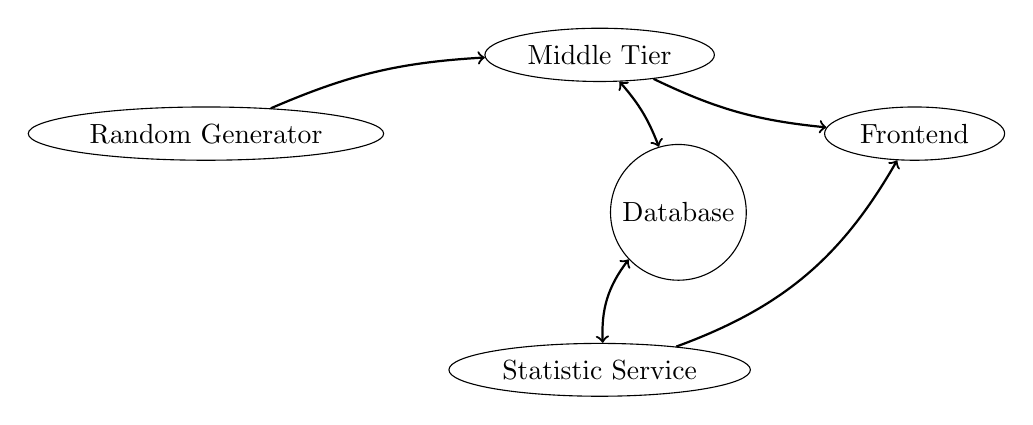
\begin{tikzpicture}
\node (A) at (0,0) [ellipse, draw] {Random Generator};
\node (B) at (5,-3) [ellipse, draw] {Statistic Service};
\node (C) at (6,-1) [circle, draw] {Database};
\node (D) at (9,0) [ellipse, draw] {Frontend};
\node (E) at (5,1) [ellipse, draw] {Middle Tier};

\draw[<->, thick] (B) to[bend left=20] (C);
\draw[->, thick] (B) to[bend right=20] (D);
\draw[->, thick] (A) to[bend left=10] (E);
\draw[->, thick] (E) to[bend right=10] (D); 
\draw[<->, thick] (E) to[bend left=10] (C);

\end{tikzpicture}

\newpage
\section{Development}
\subsection{Database}
In the further sections we will use a plain mysql docker container as a database. In order to use the Application completely locally, a local mySQL database has to be installed and a schema for the random generator application needs to be provided for a specific randgenuser.
If there is not yet a local mySQL database installed it can be done with the following command:
\begin{lstlisting}[language=Bash]
sudo apt-get update
sudo apt-get install mysql-server
\end{lstlisting}
After the installation log in to MySQL as root. 
\begin{lstlisting}[language=Bash]
sudo mysql
\end{lstlisting}
Now the Database and the user can be created and permissions to the respective schema will be given.
\begin{lstlisting}[language=SQL]
CREATE database db_example;
CREATE USER 'springuser'@'localhost' IDENTIFIED BY ThePassword;
GRANT ALL PRIVILEGES ON *.db_example TO 'springuser'@'localhost';
\end{lstlisting}
With this, the Database is ready to used by the Random Generator Example from localhost.

\subsection{Random Generator}
The Random Generator will be a verry simple Python App which has an unique Id per Service instance. It will return his id and a new Random Number. For this application we create a folder called RandGen with the following Structure.

\dirtree{%
.1 RandGen.
.2 Dockerfile.
.2 rand\_gen.py.
.2 requirements.txt.
}
The Dockerfile is needed to create the Docker Image which will be used from Kubernetes to Create the Random Generator Service.
rand\_gen.py is the complete Random Generator Python application based on Flask\footnote{More information about Flask can be found on the official Homepage \url{http://flask.pocoo.org/}}.
 \lstinputlisting[language=Python]{Applications/RandGen/rand_gen.py}
In requirements.txt are the Python packages specified. In this case it is flask. therefore this file contains only one line which is
\begin{verbatim}
Flask==1.0.2
\end{verbatim}

\subsection{Middle Tier}
The Middle Tier Application is created with Spring Initializer.
Unter the following link \url{https://start.spring.io/} Helps to bootstrap very fast a simple Spring Boot application.
In our case the fields should be filled out as followed:
\begin{tabbing}
\begin{tabular}{ll}
Project & Maven Project \\
Language & Java \\
Spring Boot & 2.1.3 (All versions would apply) \\
Group & ch.toky.randgen \\
Artifact & middletier \\
Name & MiddleTier \\
Description & Middle Tier Service for Random Generator Application \\
Packaging & Jar \\
Java Version & 8 \\
Dependencies & Web, JPA, MySQL, Rest Repositories
\end{tabular}
\end{tabbing}
The Website will create a zip file to download. This zipfile has to be extracted to the desired Project folder.
\dirtree{%
.1 middletier.
.2 Dockerfile.
.2 mvnw.
.2 mvnw.cmd.
.2 pom.xml.
.2 src.
}
all blue folders are already given. the Dockerfile still has to be created.

Now inside of the Project create the following Project Structure and files.

\dirtree{%
.1 ch.toky.randgen.middletier.
.2 MiddletierApplication.java.
.2 RandomNumber.java.
.2 ch.toky.rand-gen.middle-tier.model.
.3 PodStat.java.
.2 ch.toky.rand-gen.middle-tier.repository.
.3 PodStatRepository.java.
}
The file MiddleTierApplication.java should already be in place. as Spring Boot Initializr created this with the complete Folder structure. the packages controller, model and repository need to be created.
Inside of controller, A file named MiddletierController.java needs to be created with the following content.

Within the model package two new Files have to be created: PodStat.java and RandomNumber.java.

PodStat is an Entity and therefore the class has to be annotated with @Entity.
It contents the following fields with their respective getter and Setter Methods.
\begin{lstlisting}[language=Java]
@Id
@GeneratedValue(strategy=GenerationType.AUTO)
private Long podStatID;
private String id;
private Long timeStamp;
private Long counter;
\end{lstlisting}

The class RandomNumber is only a DTO which is retreived from the random generator Service. Therefore there is no need for a annotation.
Only the following Fields needs to be declared with their getters and setters:

\begin{lstlisting}[language=Java]
private String id;
private Long randNumber;
\end{lstlisting}

In the repository package the file PodStatRepository.java will be created.
As this java file is not a class but an interface it needs to be changed to interface and extends JpaRepository<PodStat, Long>
and it will be annotated with @Repository

Now those two methods are created 
\begin{lstlisting}[language=Java]
@Query("Select count(ps.id) from PodStat ps where ps.id = ?1")
Long countUniqueId(String id);

@Query("Select count(ps.id) from PodStat ps")
Long findMaxCount();
\end{lstlisting}

Witin the controller all the endpoints are declared. Therfore it will be annotaded with @RestController

Those fields are needed within the controller and are therefore declared first.
\begin{lstlisting}[language=Java]
@Autowired
private ObjectMapper objectMapper;
@Autowired
private PodStatRepository podStatRepository;
private Map<String, String> env = System.getenv();
\end{lstlisting}
As there should not be any hardcoded url according to the 12 Factor application \footnote{Accessible at \url{https://12factor.net/}}, the Url will be retreived through a System Variable.

Now a controller Method with the business logic can be declared:
\begin{lstlisting}[language=Java]
@RequestMapping(value = "/", produces = "application/json")
public RandomNumber getRandom() {

    RandomNumber randNum = getNewRandomNumber();
    Long maxCountId = podStatRepository.countUniqueId(randNum.getId());
    Long maxCountOverall = podStatRepository.findMaxCount();
    PodStat tmpPod = new PodStat();
    tmpPod.setId(randNum.getId());
    tmpPod.setTimeStamp(maxCountOverall+1);
    tmpPod.setCounter(maxCountId +1);
    podStatRepository.save(tmpPod);

    return randNum;

}
\end{lstlisting}
The above Method listens on the path / and returns the Random number after saving it to the database with the actual count.

Now the last Method is used to retreive the Random Number from the Random Generator Service.
\begin{lstlisting}[language=Java]
private RandomNumber getNewRandomNumber() {

    String randGenUrl=env.get("RANDOM_GENERATOR_URL");
    String URL = randGenUrl;
    RestTemplate restTemplate = new RestTemplate();

    return   restTemplate.getForObject(URL, RandomNumber.class);

}
\end{lstlisting}
Above Source code contains the Controller and the Service, which should be separated optimally.
Next two files represents POJOs which are going to be used from controller and provided by Repositories.

The last thing which needs to be done for the Middle Tier Service is to setup the default values for the Database Connection.
\begin{lstlisting}[language=Properties]
spring.jpa.hibernate.ddl-auto=update
spring.datasource.username=random_user
spring.datasource.password=random_password
spring.datasource.url=jdbc:mysql://localhost:3306/rand_numbers
\end{lstlisting}
The datasource configurations are going to be overwritten by Environment Variables once they run inside of a Docker Container.



\subsection{Statistic Service}
The Statistic Service has the same setup as the Middle Tier client.
Therefore the Project will be created too with Spring Boot initializer.
\begin{tabbing}
\begin{tabular}{ll}
Project & Maven Project \\
Language & Java \\
Spring Boot & 2.1.3 (All versions would apply) \\
Group & ch.toky.randgen \\
Artifact & stattier \\
Name & Stattier \\
Description & Statistic Tier Client for Random Generator Application \\
Packaging & Jar \\
Java Version & 8 \\
Dependencies & Web, JPA, MySQL, Rest Repositories
\end{tabular}
\end{tabbing}

\subsection{Frontend}
The frontend Application is build with Spring Boot and 

Creating Spring Boot Application:
\begin{tabbing}
\begin{tabular}{ll}
Project & Maven Project \\
Language & Java \\
Spring Boot & 2.1.3 (All versions would apply) \\
Group & ch.toky.randgen \\
Artifact & frontend \\
Name & Frontend \\
Description & Frontend Service \\
Packaging & Jar \\
Java Version & 8 \\
Dependencies & Web, Rest Repositories
\end{tabular}
\end{tabbing}


\subsection{running with Docker}

\textbf{Create a Network}
\begin{lstlisting}[language=Bash]
docker network create  -d bridge rand-gen-network
\end{lstlisting}

\textbf{Start the Database Container}

\begin{lstlisting}[language=Bash]
docker run -d --name rand-gen-database \
-e MYSQL_ROOT_PASSWORD='password' \
-e MYSQL_USER='random_user' \
-e MYSQL_PASSWORD='random_password' \
-e MYSQL_DATABASE='rand_numbers' \
--network rand-gen-network \
mysql:5.6
\end{lstlisting}

\textbf{Start the Random Generator App}
\begin{lstlisting}[language=Bash]
docker run -d --name=rand-gen-app \
--network rand-gen-network \
rand-gen-image
\end{lstlisting}

\textbf{Start the middle tier Application}
\begin{lstlisting}[language=Bash]
docker run -d \
--name middle-tier \
--network rand-gen-network \
middle-tier
\end{lstlisting}

\textbf{Starting the Stat Tier Application}
\begin{lstlisting}[language=Bash]
docker run -d \
--name stat-tier \
--network rand-gen-network \ 
stat-tier-image
\end{lstlisting}

\textbf{Start the Frontend Service}
\begin{lstlisting}[language=Bash]
docker run -d -p 8080:8080 \
--network rand-gen-network \
--name rand-frontend \
rand-frontend
\end{lstlisting}
\newpage
\section{Docker}
\subsection{Creating the Docker Images}
As we were always using multi stage builds we are now able to build the Project directly with Docker without any manual execution of some maven build commands or angular build commands.
It is mostly important for the build from our Frontend, as we do not need to run ng build and after that mvn clean package.
With this we can also always be sure to have the latest version of the jar file, as we are building the jar together with the Docker Image.

There is one huge disadvantage. As every docker Container has its own environment and we cannot mount a hostpath during the build, we need to download all the dependencies for each build which takes quite some time.

As our builds will run every time in a new Container, it needs to load all dependencies each time we are going to build the Project. This takes a lot of time and there are pluginswhich makes this much easier.
For example the spotify docker Maven plugin which would enable us to build the Dockerfile directly with maven \footnote{https://github.com/spotify/docker-maven-plugin}.
There is also a maven plugin to execute the angular build before building the jar file \footnote{https://github.com/eirslett/frontend-maven-plugin}.
All of them can make our life easier but as we want to dive a little bit deeper into Docker, we will do it wit plain Dockerfiles.

\textbf{Create Random Generator}

The Dockerfile to create the Docker image:
\lstinputlisting[language=Bash]{Applikationen/generator/Dockerfile}

within the root directory of the Random Generator.

the flag -t inicates that the name of the image and the dot at the end tells docker to use the Dockerfile from the current working directory.

\begin{lstlisting}[language=Bash]
docker build -t rand-gen-image .
\end{lstlisting}

\textbf{Middle Tier Docker Image}
\lstinputlisting[language=Bash]{Applikationen/middletier/Dockerfile}

We are using anapsix base image, as we want to keep the Docker image as small as possible.

Finally we can create the docker image with the following Command.

Important is, we need to be in the root directory of the Projecct where also the Dockerfile is stored.
\begin{lstlisting}[language=Bash]
docker build -t rand-middle-image .
\end{lstlisting}
As previously mentioned, we will use multi stage builds. In this case we use a maven base image as a builder.
Reference for using maven with Docker \url{https://hub.docker.com/_/maven/}

\textbf{Statistic Service}
For the image itself we are using anapsix base image as this is currently the smallest possible java base image \url{https://hub.docker.com/r/anapsix/alpine-java/dockerfile/}
If you want to run the project on a raspberry, you would need to change the base image to hypriot as a Raspberry has a diffret underlaying CPU architecture which is based on ARM \footnote{https://github.com/hypriot/rpi-java}



\lstinputlisting[language=Bash]{Applikationen/statservice/Dockerfile}

Basically the Dockerfile for this Service looks pretty much the same as the one for the Middle tier except that we do not need to declare an environment variable for the random generator.

\begin{lstlisting}[language=Bash]
docker build -t rand-stat-image .
\end{lstlisting}

\textbf{Frontend Service}

As we have one more step within the Frontend service. We need to have one more stage. As we need node package manager to build the angular application we are goint to use a node.js docker base image \footnote{ Node Repository Docker hub \url{https://hub.docker.com/_/node/}}.


\lstinputlisting[language=Bash]{Applikationen/frontend/Dockerfile}

\begin{lstlisting}[language=Bash]
docker build -t rand-front-image .
\end{lstlisting}


\subsection{running with Docker}

\textbf{Create a Network}
\begin{lstlisting}[language=Bash]
docker network create  -d bridge rand-network
\end{lstlisting}

\textbf{Start the Database Container}

\begin{lstlisting}[language=Bash]
docker run -d --name rand-gen-database \
-e MYSQL_ROOT_PASSWORD='password' \
-e MYSQL_USER='random_user' \
-e MYSQL_PASSWORD='random_password' \
-e MYSQL_DATABASE='rand_numbers' \
--network rand-network \
mysql:5.6
\end{lstlisting}

\textbf{Start the Random Generator App}
\begin{lstlisting}[language=Bash]
docker run -d --name=rand-gen-tier \
--network rand-network \
rand-gen-image
\end{lstlisting}

\textbf{Start the middle tier Application}
\begin{lstlisting}[language=Bash]
docker run -d \
--name rand-middle-tier \
--network rand-network \
middle-tier
\end{lstlisting}

\textbf{Starting the Stat Tier Application}
\begin{lstlisting}[language=Bash]
docker run -d \
--name rand-stat-tier \
--network rand-network \ 
rand-stat-image
\end{lstlisting}

\textbf{Start the Frontend Service}
\begin{lstlisting}[language=Bash]
docker run -d -p 8080:8080 \
--network rand-network \
--name rand-frontend \
rand-front-image
\end{lstlisting}

All the default environment Variables are already set within the Dockerfiles therefore we can startup all the services one by one.

\newpage
\section{Kubernetes}
\subsection{Installing Kubernetes}


To play arround and get to know Kubernetes it is recommendet to install minikube \footnote{\url{https://kubernetes.io/docs/tasks/tools/install-minikube/}} which is running inside a VM on your local machine.
If you want to use Kubernetes on a Server and deploy PROD ready application then you have the option to rent directly a Kubernetes Cluster from a Vendor
\begin{itemize}
\item AWS EKS \url{https://aws.amazon.com/de/eks/}
\item GKE Google Cloud \url{https://cloud.google.com/kubernetes-engine/}
\item IBM Kubernetes Service \url{https://www.ibm.com/cloud/container-service}
\end{itemize}

You can also install Kubernetes on a plain server, we use ubuntu for this setup. weh use the following instruction to get this done \footnote{\url{https://linuxconfig.org/how-to-install-kubernetes-on-ubuntu-18-04-bionic-beaver-linux}}
 But first we need to add the Kubernetes to our installation repository.
\begin{verbatim}
curl -s https://packages.cloud.google.com/apt/doc/apt-key.gpg \ 
| sudo apt-key add
\end{verbatim}

\begin{verbatim}
sudo apt-add-repository \
"deb http://apt.kubernetes.io/ kubernetes-xenial main"
$ sudo apt install kubeadm 
\end{verbatim}

\begin{verbatim}
sudo swapoff -a
\end{verbatim}

Now we have Kubeadm installed, we can continue with the server setup based on the instruction from Kubernetes itself \footnote{\url{https://kubernetes.io/docs/setup/independent/create-cluster-kubeadm/}}

The pod network will be Callico.

\begin{verbatim}
kubeadm init --apiserver-advertise-address=<ip-address> \
--pod-network-cidr=192.168.0.0/16
\end{verbatim}

Switch back to non root user and execute those commands.

\begin{verbatim}
mkdir -p $HOME/.kube
sudo cp -i /etc/kubernetes/admin.conf $HOME/.kube/config
sudo chown $(id -u):$(id -g) $HOME/.kube/config
\end{verbatim}

/proc/sys/net/bridge/bridge-nf-call-iptables to 1

Now we just need to deploy the pod network.
\begin{verbatim}
kubectl apply -f \
https://docs.projectcalico.org/v3.3/getting-started/
kubernetes/installation/hosted/rbac-kdd.yaml
kubectl apply -f \
https://docs.projectcalico.org/v3.3/getting-started/
kubernetes/installation/hosted/
kubernetes-datastore/calico-networking/1.7/calico.yaml
\end{verbatim}

Wait until all pods are up and running.
kubectl get pods --all-namespaces

If we are using a single node cluster, we need to tell Kubernetes that it is allowed to deploy pods on the master node (which is the only node in the cluster)
\begin{verbatim}
kubectl taint nodes --all node-role.kubernetes.io/master-
\end{verbatim}

Now we are done with the setup and we can start deployin pods to the Kubernetes cluster.

\subsection{Deploy Services}

\textbf{Kubernetes Commands}

Kubernetes is managing all entities according to specifications. Which means we need to declarare our desired state and kubernetes will do all the magig for us and it will also constantly check if the actual state is matching with the desired state and adjust if neccessary.
kubectl is used to configure kubernetes \footnote{\url{https://kubernetes.io/docs/reference/kubectl/overview/}}.
in our case we deslare all our desired states within yaml files and post them via \texttt{kubectl create -f <filename.yml>} to kubernetes.
the create command means that the declared ressources in the yaml file $Deployment$, $Service$, $Secret$, $ConfigMap$ needs to be created. the $-f$ flag means it should read it from the following file.

after that we can user \texttt{kubectl get pods} to show the all pods within the default namespace and \texttt{kubectl get svc} to show all services.


\textbf{Configuration}

\textbf{Secrets}
As Secrets\footnote{\url{https://kubernetes.io/docs/tasks/inject-data-application/distribute-credentials-secure/}} can only store base64 encoded values, we need to convert all our values with base64 with the following commands:
\begin{verbatim}
echo -n 'random_user' | base64
echo -n 'random_password' | base64
echo -n 'password' | base64
\end{verbatim}
and then save the result in the secrets file as shown below.
Secret file with values for the whole application.
\lstinputlisting[language=Bash]{config-files/secret.yml}

Environment Variable configuration for the whole application.
\lstinputlisting[language=Bash]{config-files/config-env.yml}

All the Applications are running inside of a docker container and managed within a Kubernetes Pod and accessible via a Kubernetes Service where only the Frontend Service is bound to a Node Port.

\textbf{Database}
A database is always quite special for a deployment as the whole Container setup is meant to run stateless. Which means all the data is lost once a container dies. Mostly this is very bad for a database as there all the relevant data should be persisted.

Docker itself provides therefore persistent Volumens which can be mounted by a Container.

Within Kubernetes we create therefore a PersistentVolume \footnote{\url{https://kubernetes.io/docs/concepts/storage/persistent-volumes/}} to request a persisten Volume. Kubernetes will then search for a persistent Volume which would satisfie the requirements from the claim and allocates it to the claim.

A pod can then be linked to a persistent volume via the persistent volume claim.
In the following yaml file we declare first a Persistent volume and afterwards the persistent volume claim.
\lstinputlisting[language=Bash]{config-files/pv-example/pv-claim.yml}

Within the pod we would then link the pod to the pv claim via the following arguments within the containers: argument from the mysql deployment.
\lstinputlisting[language=Bash]{config-files/pv-example/pod-pv-claim.yml}
Nevertheless, this is not realy required for our application because we only need the database as a provisional storage.

A more detailed example from Kubernetes can be found under this link \url{https://kubernetes.io/docs/tasks/configure-pod-container/configure-persistent-volume-storage/}

Deployment
\lstinputlisting[language=Bash,firstline=16]{config-files/database.yml}

As a pod can always vary its ip adress, we need to have a stable endpoint to access the pods.
Specificly for this purpose, kubernetes provides services.
Service to make the Database Pod available 
\lstinputlisting[language=Bash,lastline=13]{config-files/database.yml}

\textbf{Random Generator}
Now we also declare the deployment for the generator service.
Notice that we have two replicas for the generator. this is because we wand to have two diffrent ids as a source for our generator.
\lstinputlisting[language=Bash,firstline=17]{config-files/generator.yml}

The corresponsing service.
\lstinputlisting[language=Bash,lastline=14]{config-files/generator.yml}

\textbf{Middle Tier service}
\lstinputlisting[language=Bash,firstline=17]{config-files/middle-tier.yml}
The service
\lstinputlisting[language=Bash,lastline=14]{config-files/middle-tier.yml}

\textbf{Statistic Service}
\lstinputlisting[language=Bash,firstline=17]{config-files/stat-tier.yml}
Service
\lstinputlisting[language=Bash,lastline=14]{config-files/stat-tier.yml}

\textbf{Frontend}
\lstinputlisting[language=Bash,firstline=18]{config-files/frontend.yml}

Service:
\lstinputlisting[language=Bash,lastline=15]{config-files/frontend.yml}




\end{document}